% This must be in the first 5 lines to tell arXiv to use pdfLaTeX, which is strongly recommended.
\pdfoutput=1
% In particular, the hyperref package requires pdfLaTeX in order to break URLs across lines.

\documentclass[11pt]{article}

% Remove the "review" option to generate the final version.
\usepackage{ACL2023}

\usepackage{graphicx}
\usepackage{float}
% Standard package includes
\usepackage{times}
\usepackage{latexsym}

% For proper rendering and hyphenation of words containing Latin characters (including in bib files)
\usepackage[T1]{fontenc}
% For Vietnamese characters
% \usepackage[T5]{fontenc}
% See https://www.latex-project.org/help/documentation/encguide.pdf for other character sets

% This assumes your files are encoded as UTF8
\usepackage[utf8]{inputenc}

% This is not strictly necessary, and may be commented out.
% However, it will improve the layout of the manuscript,
% and will typically save some space.
\usepackage{microtype}

% This is also not strictly necessary, and may be commented out.
% However, it will improve the aesthetics of text in
% the typewriter font.
\usepackage{inconsolata}


% If the title and author information does not fit in the area allocated, uncomment the following
%
%\setlength\titlebox{<dim>}
%
% and set <dim> to something 5cm or larger.

\title{NNTI Project WiSe 2025}

% Author information can be set in various styles:
% For several authors from the same institution:
% \author{Author 1 \and ... \and Author n \\
%         Address line \\ ... \\ Address line}
% if the names do not fit well on one line use
%         Author 1 \\ {\bf Author 2} \\ ... \\ {\bf Author n} \\
% For authors from different institutions:
% \author{Author 1 \\ Address line \\  ... \\ Address line
%         \And  ... \And
%         Author n \\ Address line \\ ... \\ Address line}
% To start a seperate ``row'' of authors use \AND, as in
% \author{Author 1 \\ Address line \\  ... \\ Address line
%         \AND
%         Author 2 \\ Address line \\ ... \\ Address line \And
%         Author 3 \\ Address line \\ ... \\ Address line}

\author{ Abdelsalam Helala \\
  7056985 \\\And
  Mostafa Hammouda \\
  7058050 \\\And
  Loulwah Arnaout \\
    7062523 \\}

\begin{document}
\maketitle
\begin{abstract}
This project aims to enhance the performance of a pre-trained chemical language model for predicting lipophilicity. The project is divided into three tasks: Task 1 involves fine-tuning the model on the Lipophilicity dataset and applying MLM as unsupervised fine-tuning, Task 2 explores the use of influence functions to select high-impact external data points for further training, and Task 3 examines alternative data selection strategies and parameter-efficient fine-tuning methods. The results from these tasks aim to optimize the model's performance on the target dataset, leveraging both external data and advanced training techniques.
\end{abstract}

\section{Task 1}
\subsection{Fine-tune a Chemical Language Model on Lipophilicity}
We begin by loading the necessary libraries, including in addition to those previously loaded in the template, \texttt{scikit-learn} \cite{scikit-learn} for data splitting and evaluation metrics, and \texttt{matplotlib} \cite{Hunter:2007} for visualizing the training and evaluation loss curves.

We use a dataset consisting of SMILES strings representing molecules, alongside their corresponding lipophilicity values. The SMILESDataset class is implemented to tokenize the SMILES strings using the pre-trained tokenizer from HuggingFace's \texttt{Transformers} library \cite{Wolf2020Transformers}, and pad them to ensure uniform input length for the model.

The dataset is split into training ($80\%$) and testing ($20\%$) sets. For this task, we use a batch size of 16, resulting in a total of 210 training batches and 53 test batches.

Next, we load a pre-trained MoLFormer model from HuggingFace and extend it with a regression head suitable for predicting continuous numeric values (lipophilicity). We train the model using mean squared error (MSE) as the loss function (suitable for regression tasks) and Adam as the optimizer \cite{Kingma2014Adam} for optimizing the model parameters.

During training, we monitor and observe the training and evaluation losses for 20 epochs and decide to stop the training at 8 epochs, where the evaluation loss stabilizes, while the training loss continues to decrease. This suggests that the model has started overfitting. The following plot, not included in the notebook, shows what we observed: 
\begin{figure}[ht]
  \centering
  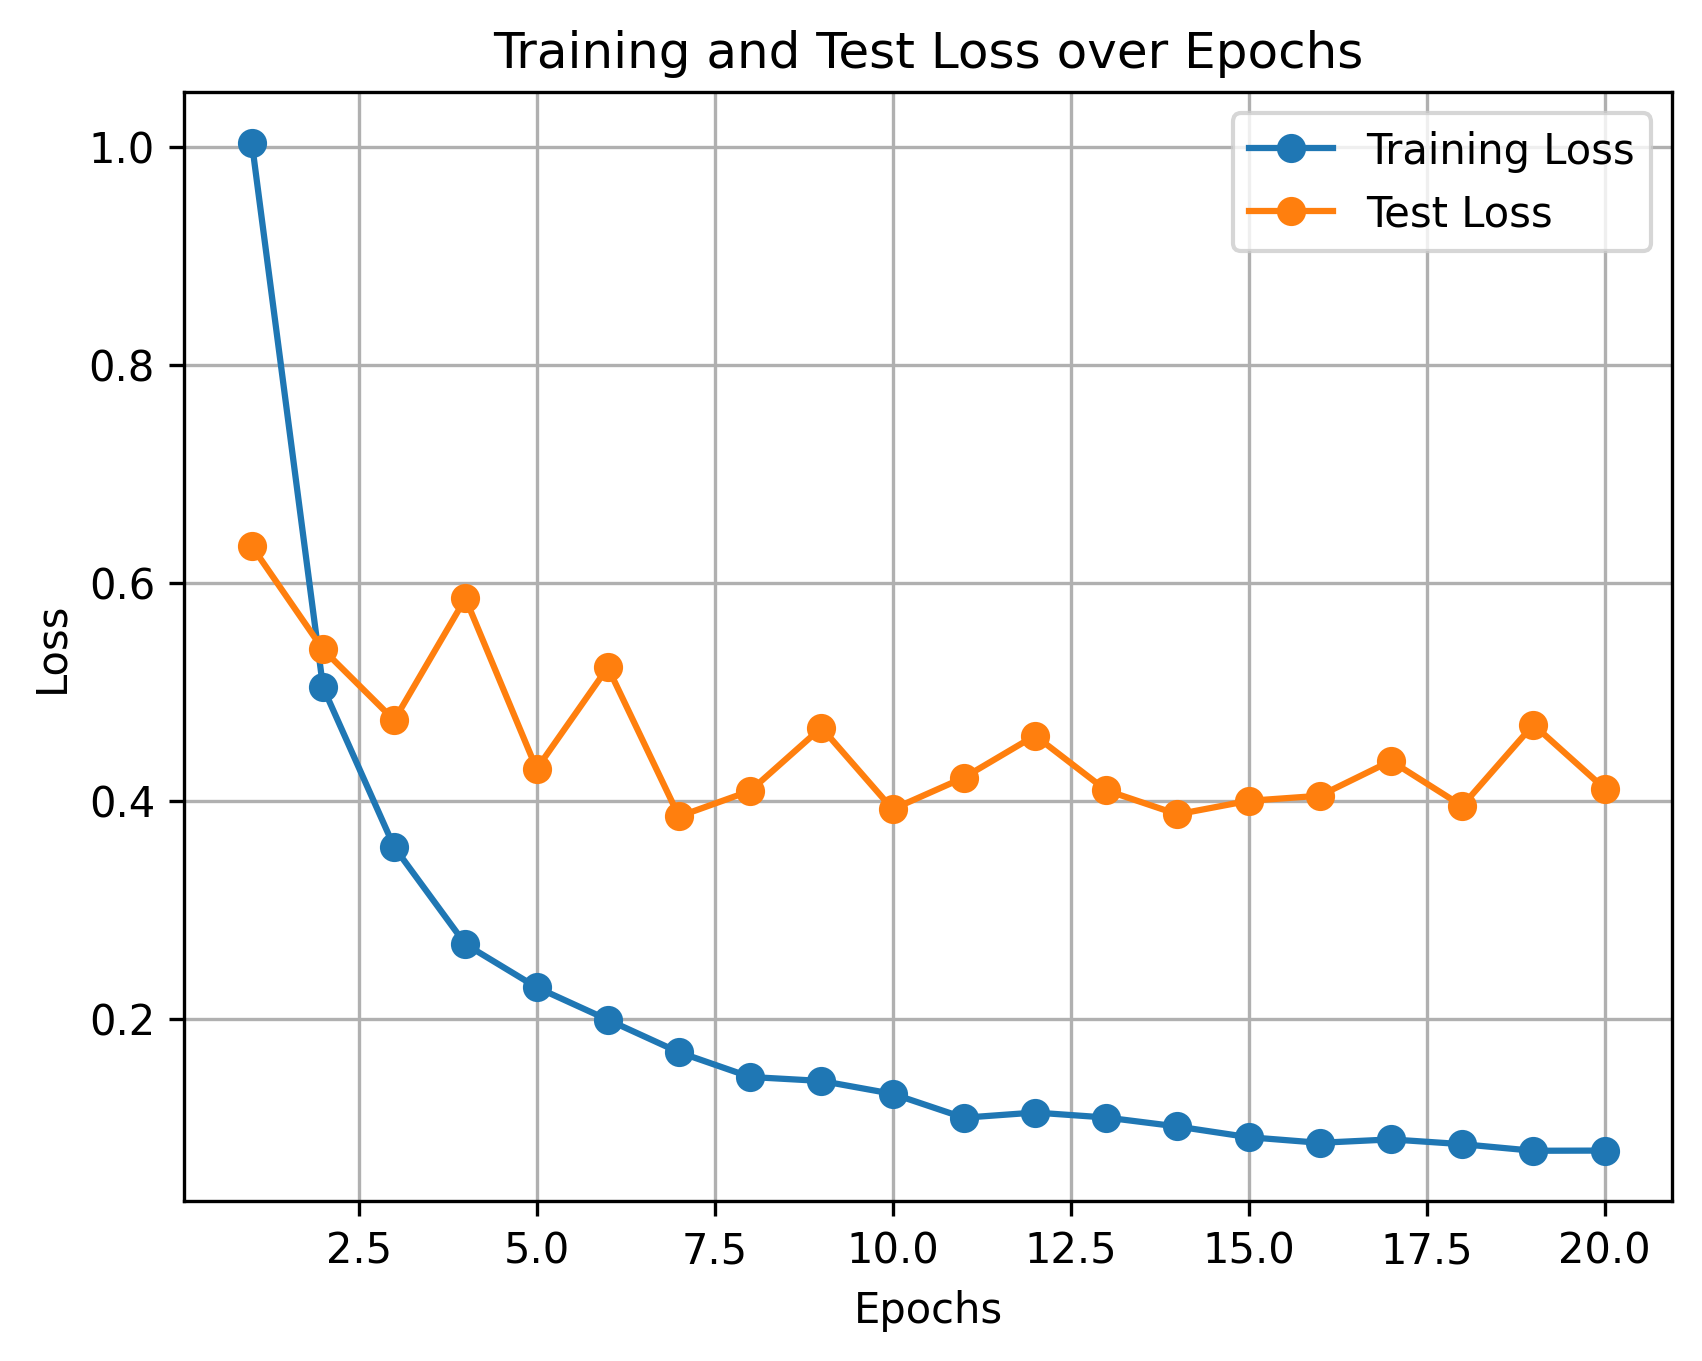
\includegraphics[width=0.45\textwidth]{images/1.training_loss_plot.png}
  \caption{Training vs. evaluation loss over 20 epochs.}
  \label{fig:results}
\end{figure}

We then evaluate the performance on the test set using mean squared error (MSE), mean absolute error (MAE), and $R^2$ score.
\subsection{Add Unsupervised Finetuning}
In the second part of the task, we fine-tune the model using Masked Language Modeling (MLM), a common pre-training task in transformer models. For this, we mask a proportion of tokens in the SMILES strings, and train the model to predict the original tokens.
The MLMDataset class is designed to handle this masked input format, similar to the SMILESDataset class. In this class, each sample is returned with a masked token sequence, and the label is the unmasked version of the sequence.
We train the same pre-trained model as before on the masked data for 20 epochs using cross-entropy loss as it is a natural fit for this classification task. AdamW is again used as the optimizer. The model is saved after fine-tuning and used for downstream tasks.
\subsection{Fine-tune for Comparison}
In the final step, we add a regression head to the unsupervised fine-tuned model and train it for 8 epochs, with training stopping when the evaluation loss stabilizes.
\begin{figure}[ht]
  \centering
  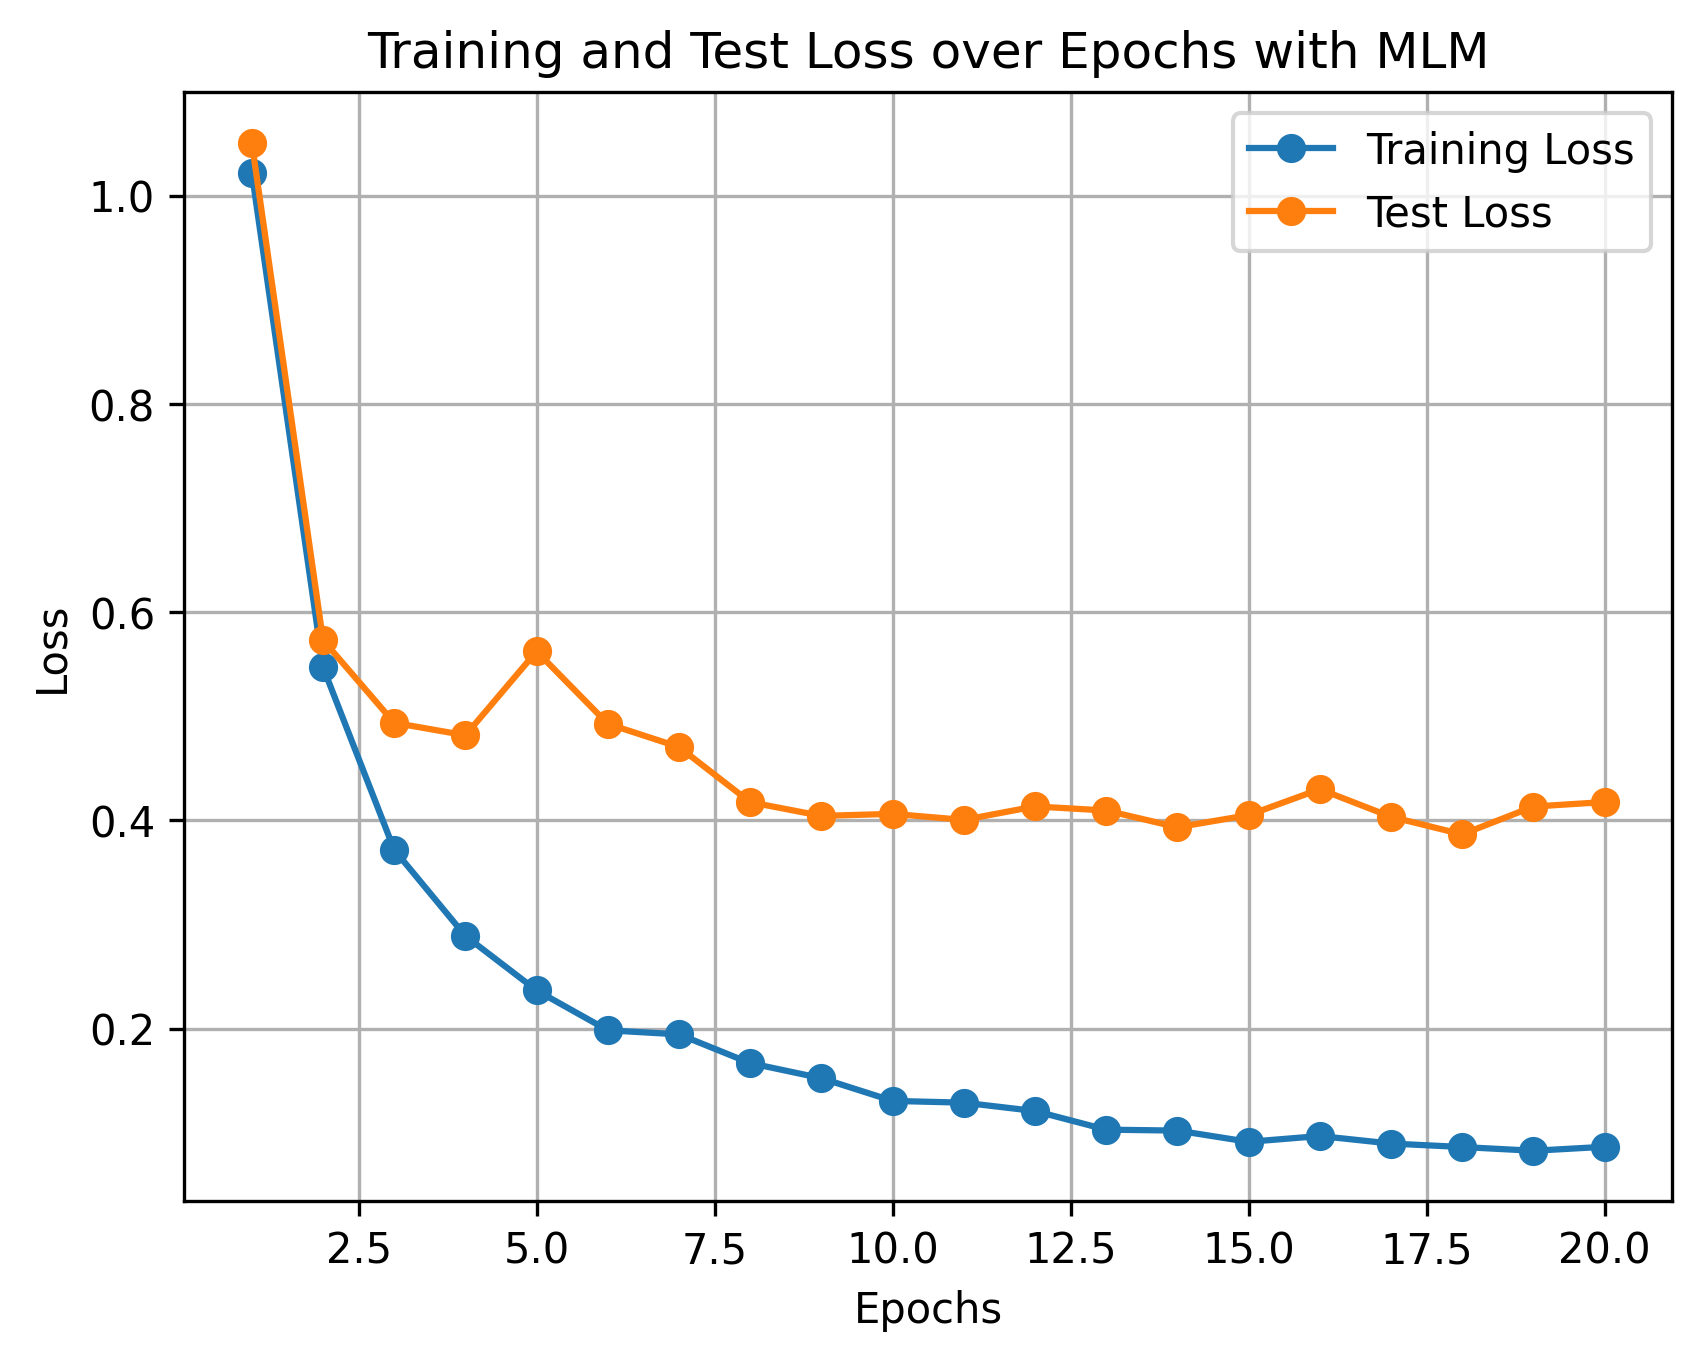
\includegraphics[width=0.45\textwidth]{images/1.training_loss_plot_mlm.png}
  \caption{Training vs. evaluation loss over 20 epochs.}
  \label{fig:results}
\end{figure}
We can notice a smoother decrease and stabilization of the test loss in this model than in the non-fine-tuned one.
When comparing the training loss of the two models, we can see how the one corresponding to the MLM-fine-tuned model is consistently lower across epochs:
\begin{figure}[ht]
  \centering
  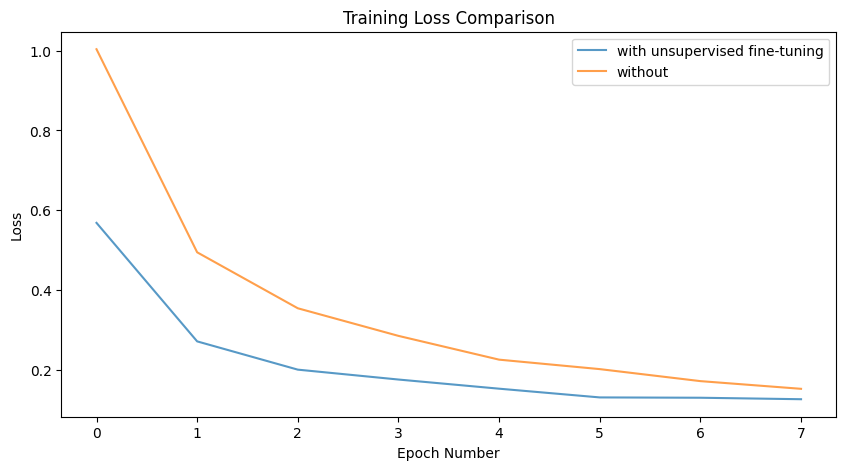
\includegraphics[width=0.45\textwidth]{images/1.training_loss_comparison.png}
  \caption{Training loss of both models across epochs.}
  \label{fig:results}
\end{figure}
We evaluate the model on the test set, then compare its performance with that of the model without unsupervised fine-tuning:
\begin{table}[ht]
\centering
\begin{tabular}{lcc}
\hline
\textbf{Metric} & \textbf{Without} & \textbf{With} \\
\hline
\textbf{MSE} & 0.472255 & 0.425943 \\
\textbf{MAE} & 0.531588 & 0.494172 \\
\textbf{R2}  & 0.680363 & 0.711709 \\
\hline
\end{tabular}
\caption{Model performance metrics without and with unsupervised fine-tuning.}
\label{tab:metrics_comparison}
\end{table}
We notice an improvement in model performance, as evidenced by the lower MSE, MAE, and higher R² scores.


\section{Task 2}

\subsection{Data Preparation}
After importing the same libraries loaded in task 1, we loaded the provided external dataset and performed Tokenization by using a pretrained tokenizer which convert molecular structures into a machine-readable format.

\subsection{Gradient Computation}
Then we defined the gradient computation function which calculates gradients by performing backpropagation of the loss through the model, which shows the influence of each parameter on the prediction.

\subsection{LiSSA Approximation}
The LiSSA algorithm \cite{agarwal2017secondorderstochasticoptimizationmachine} is used to approximate the inverse Hessian-vector product, which is important for efficient influence computation. The following steps shows how it works:

\begin{itemize}
    \item First we compute the gradient of the loss with respect to the model parameters.
    \item Then with an iterative approach, the Hessian-vector product is approximated over several iterations and at each iteration we refined the estimation by adjusting the dampening factor and scaling parameter to ensure convergence and stability.
    \item Finally the process culminates in an approximate inverse Hessian-vector product, which will be used for influence calculation.
\end{itemize}

\subsection{Influence Score Calculation}
We refer to \cite{koh2020understandingblackboxpredictionsinfluence} on influence functions to calculate and log the influence scores for all samples in the external dataset. The calculation is done by:

\begin{itemize}
    \item First using the approximated inverse Hessian-vector product from the LiSSA algorithm.
    \item and then multiplying this with the gradient of the test loss to estimate how removing a data point would influence the overall loss.
    \item When we get a high influence score this means that it has a high impact on the model's predictions, which will help identify significant data points.
\end{itemize}

\subsection{Data Filtering and Saving}
After computing the influence scores, we filtered the data points to use only the most impactful ones by:

\begin{itemize}
    \item Ranking them by their influence scores.
    \item Selecting the top 50 percent.
    \item Saving them to a CSV file for the model training.
\end{itemize}


\subsection{Results}
Now we will compare our models performance with the models in task 1 that was done without and with unsupervised finetuning. We used the same learning rate and number of epochs. 

First the loss plot shows that the model is converging after 8 epochs, and neither underfitting nor overfitting. Secondly the results in table 2 show that the  Influence Function-based Data Selection approach has better results and performance than the models in task 1 as evidenced by the lower MSE, MAE, and higher R² scores.

\begin{figure}[ht]
  \centering
  \includegraphics[width=0.45\textwidth]{images/train_eval_loss_comparison.png}
  \caption{Training and evaluation loss comparison across epochs.}
  \label{fig:results}
\end{figure}
We evaluate the model on the test set, then compare its performance with both models in task 1 with and without unsupervised fine-tuning:
\begin{table}[ht]
\centering
\begin{tabular}{lccc}
\hline
\textbf{Metric} & \textbf{With} & \textbf{Without} & \textbf{IFDS} \\
\hline
\textbf{MSE} & 0.4722 & 0.4259 & 0.3945 \\
\textbf{MAE} & 0.5315 & 0.4941 & 0.4772 \\
\textbf{R2}  & 0.6803 & 0.7117 & 0.7330 \\
\hline
\end{tabular}
\caption{Model performance metrics without and with unsupervised fine-tuning in task 1 compared to Influence Function-based Data Selection IFDS model performance metrics in task 2.}
\label{tab:metrics_comparison}
\end{table}


\subsection{Conclusion}
When we trained the model using Influence Function based Data Selection approach, the predictive performance and loss were better than the baseline in task 1.

\section{Task 3} 
\subsection{Introduction}
This task investigates parameter-efficient fine-tuning techniques. Instead of updating all model parameters (which is computationally expensive), we experiment with strategies that modify only specific parts of the model (BitFit, LoRA, and IA3). These methods allow us to efficiently adapt a pre-trained model to our dataset while preserving generalization and minimizing unnecessary updates.
\subsection{Code Implementation}
The provided code follows a structured pipeline consisting of:
\begin{enumerate}
  \item \textbf{Model and Dataset Setup}
  
    The starting point is the same pre-trained model and tokenizer as tasks 1 and 2, and the external dataset used for task 2.
\item \textbf{Data Splitting Strategy}
\begin{itemize}
    \item 80\% training and 20\% evaluation
    \item Labels were binarized using the mean value as a threshold.
\end{itemize}
\item \textbf{Fine-Tuning Strategies Implemented}
Instead of full fine-tuning, we applied three parameter-efficient approaches:

\textbf{BitFit}
\begin{itemize}
    \item Updates only bias parameters of the model.
    \item All other weights remain frozen.
    \item Low memory usage and faster training.
\end{itemize}

\textbf{LoRA (Low-Rank Adaptation)}
\begin{itemize}
    \item Introduces learnable low-rank matrices into the query and value layers.
    \item Set rank \( r = 8 \), scaling factor \( \alpha = 16 \).
    \item Efficient adaptation while keeping most of the model unchanged.
\end{itemize}

\textbf{IA3 (Implicit Adaptive Adjustment)}
\begin{itemize}
    \item Scales activations in specific layers.
    \item Uses multiplicative scaling factors instead of modifying weights.
    \item Aims to efficiently adapt the model without excessive computations.
\end{itemize}

\item \textbf{Training Configuration}
Each method was trained with different hyperparameters:
\begin{table}[ht]
\centering
\begin{tabular}{lcc}
\hline
\textbf{Strategy} & \textbf{Epochs} & \textbf{Learning Rate} \\
\hline
BitFit & 30 & \(2 \times 10^{-5}\) \\
LoRA  & 20 & \(1 \times 10^{-5}\) \\
IA3   & 20 & \(5 \times 10^{-6}\) \\
\hline
\end{tabular}
\caption{Training Hyperparameters for Different Fine-Tuning Strategies}
\label{tab:hyperparameters}
\end{table}

Training was logged in WandB, and models were saved after training.
\end{enumerate}
\subsection{Interpretation of W\&B Graphs}
\textbf{Evaluation Steps Per Second}: BitFit is the fastest in evaluation, while LoRA is the slowest, possibly due to additional computations.

        \begin{figure}[H]
      \centering
      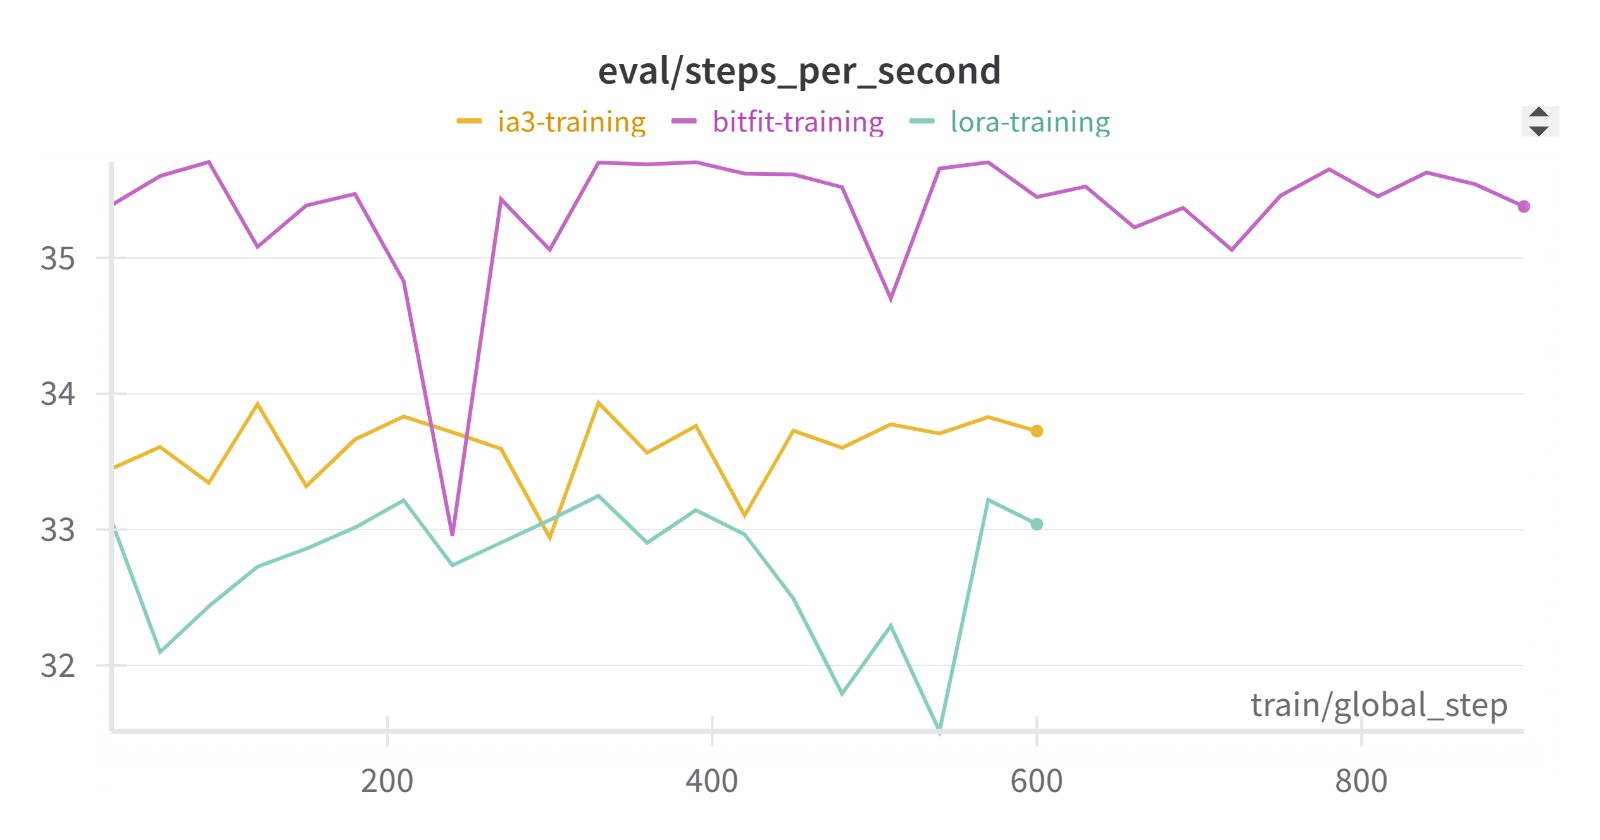
\includegraphics[width=0.45\textwidth]{images/3.eval_steps_per_sec.jpg}
      \caption{Evaluation step/second of the 3 strategies.}
      \label{fig:results}
    \end{figure}
\textbf{Evaluation Loss (BitFit)}: Loss decreases initially but stabilizes with minor fluctuations, suggesting effective fine-tuning.

    \begin{figure}[H]
  \centering
  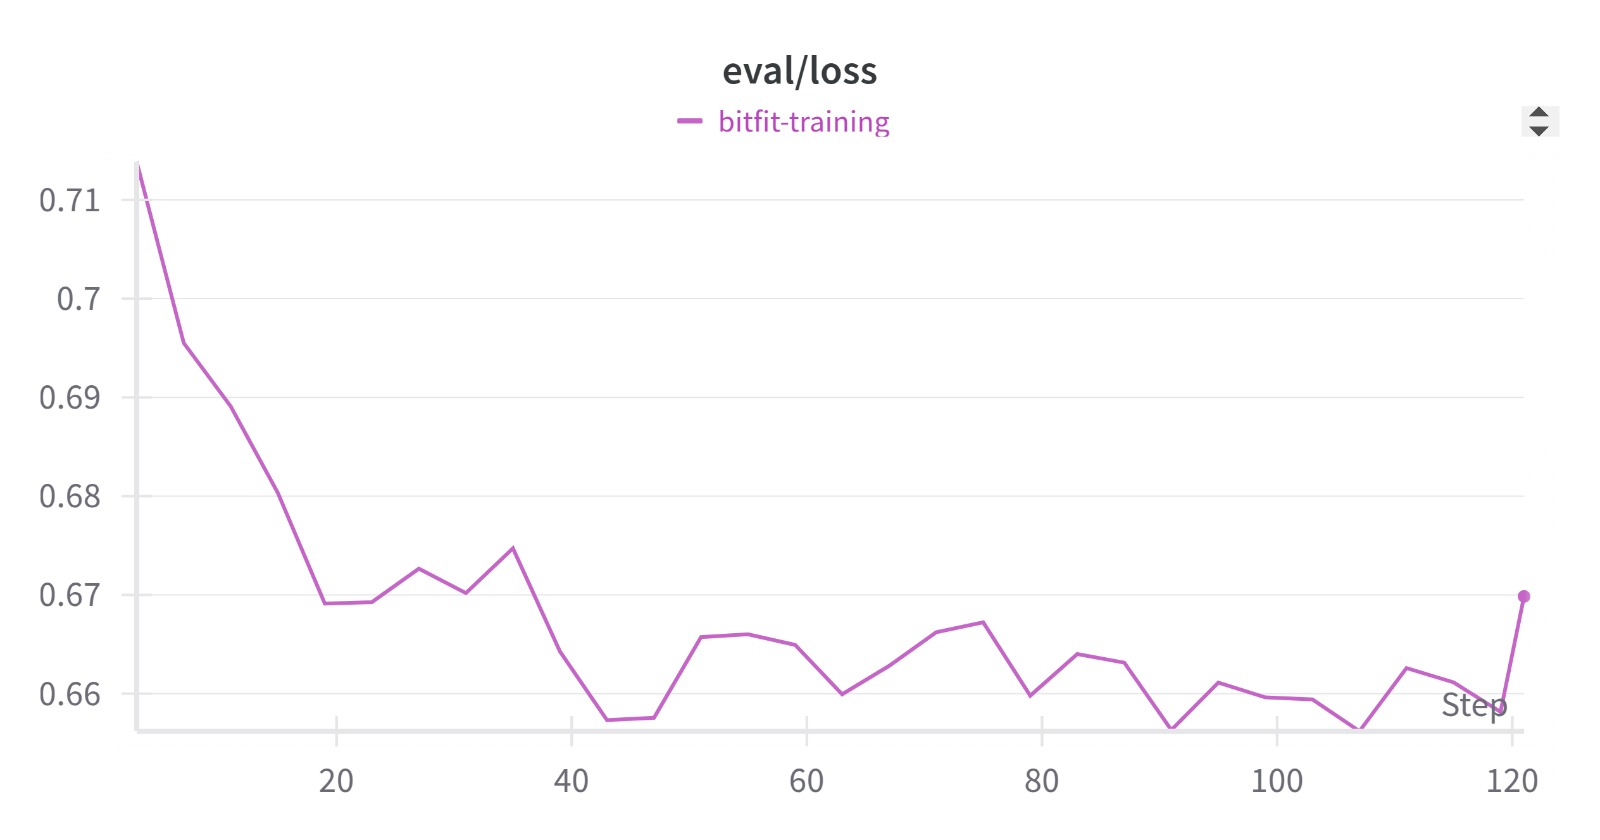
\includegraphics[width=0.45\textwidth]{images/3.eval_loss_bitfit.jpg}
  \caption{Evaluation loss BitFit.}
  \label{fig:results}
\end{figure}    
\textbf{Evaluation Runtime}: LoRA takes the longest, likely due to extra matrix computations; BitFit and IA3 are more efficient.

    \begin{figure}[H]
  \centering
  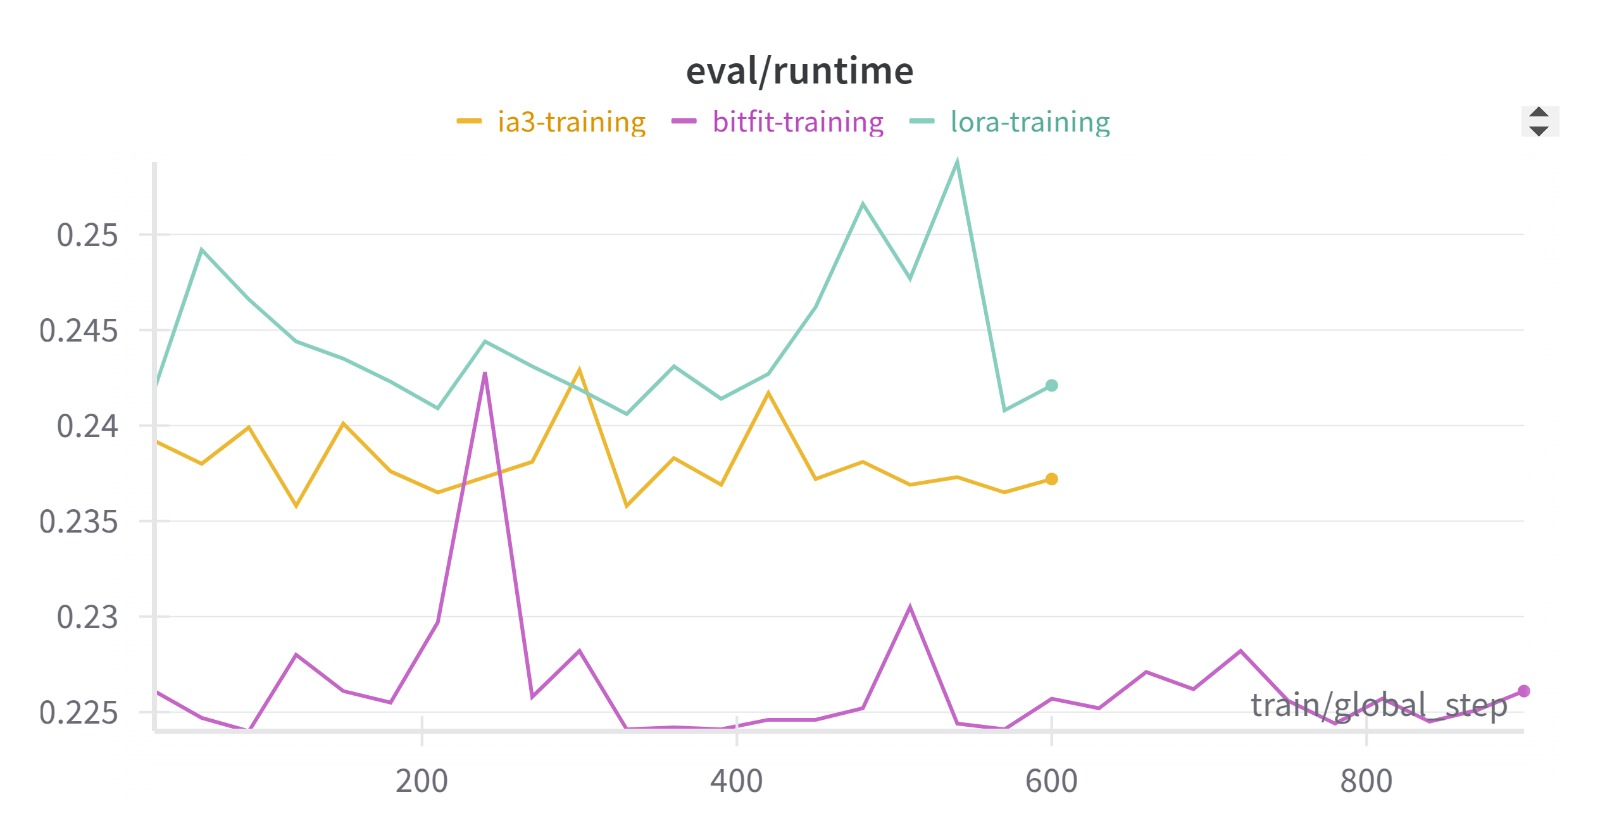
\includegraphics[width=0.45\textwidth]{images/3.eval_runtime.jpg}
  \caption{Evaluation runtime comparison.}
  \label{fig:results}
\end{figure}
\textbf{Gradient Norm}: IA3 had the lowest gradient norm, indicating stable weight updates, whereas BitFit and LoRA had more fluctuations.

    \begin{figure}[H]
  \centering
  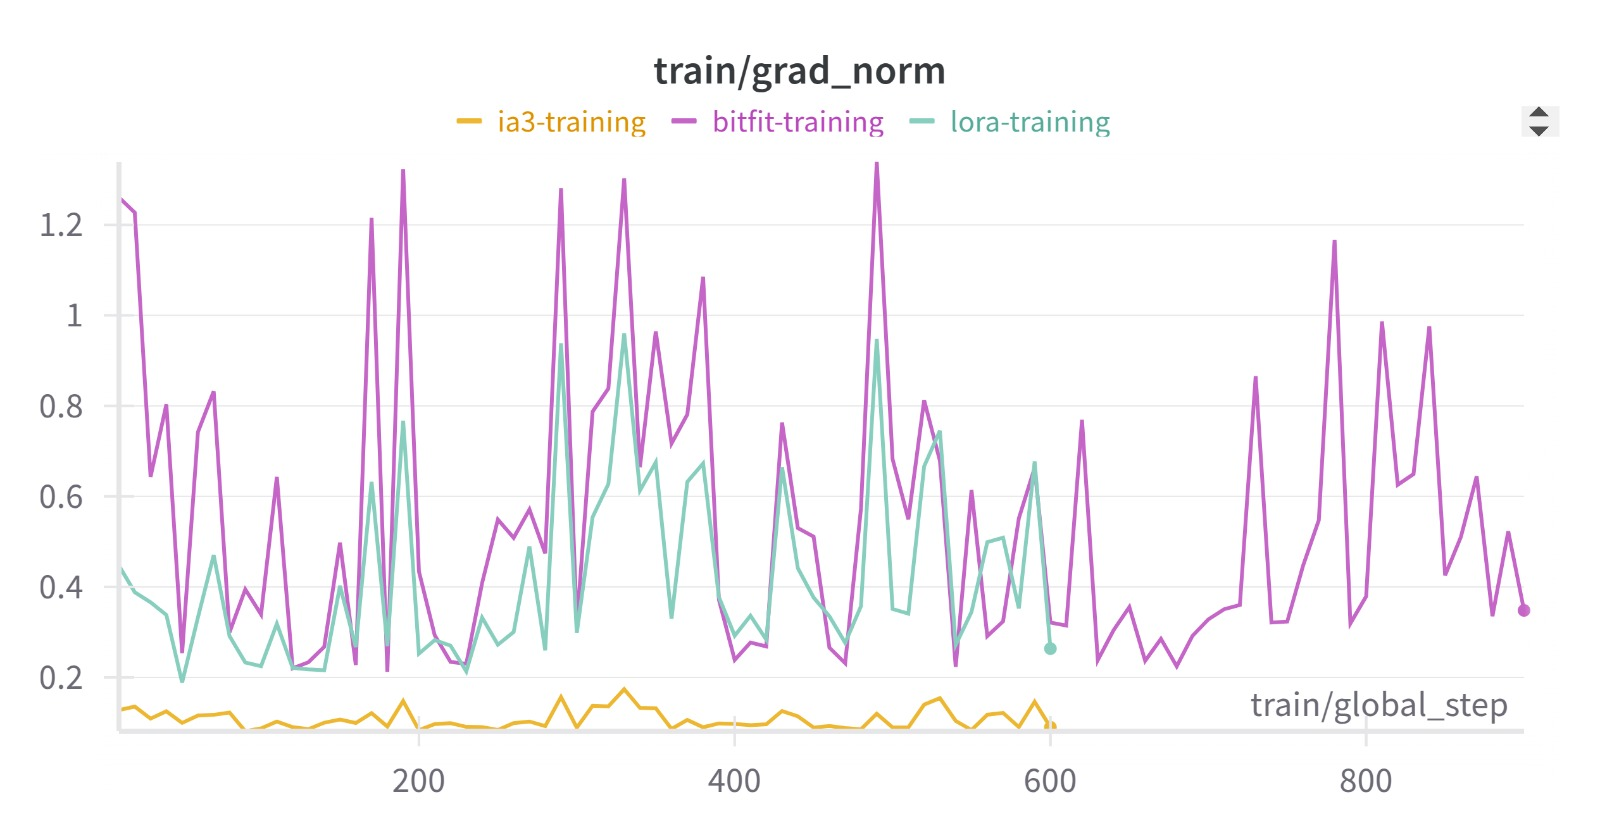
\includegraphics[width=0.45\textwidth]{images/3.train_gradnorm.jpg}
  \caption{Gradient Norm comparison.}
  \label{fig:results}
\end{figure}
\textbf{Training Loss}: BitFit achieved the lowest training loss, while IA3 had the highest, indicating less effective fine-tuning.

        \begin{figure}[H]
  \centering
  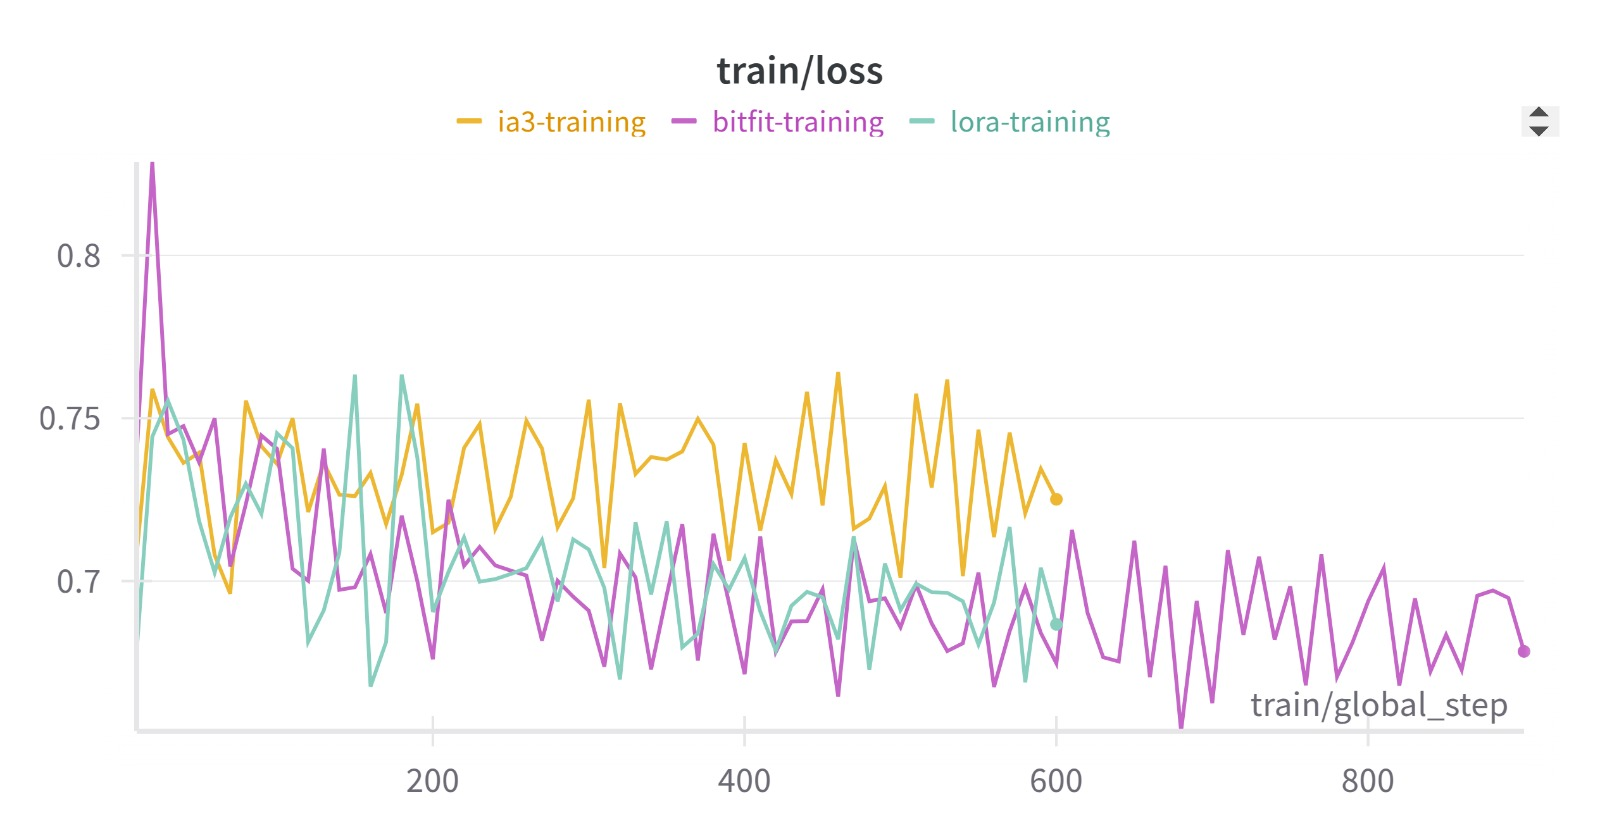
\includegraphics[width=0.45\textwidth]{images/3.train_loss.jpg}
  \caption{Train loss comparison.}
  \label{fig:results}
\end{figure}

\subsection{Performance Comparison}
\begin{itemize}
    \item BitFit is the most computationally efficient and achieves the best evaluation loss.
    \item LoRA requires more computational resources but allows for greater adaptability.
    \item IA3 is lightweight but does not improve loss significantly.
\end{itemize}
% Entries for the entire Anthology, followed by custom entries
\bibliography{custom}
\bibliographystyle{acl_natbib}
\end{document}
